%%\documentclass[a4paper,12pt,oneside]{llncs}
\documentclass[12pt,letterpaper]{article}
\usepackage[right=2cm,left=3cm,top=2cm,bottom=2cm,headsep=0cm]{geometry}

%%%%%%%%%%%%%%%%%%%%%%%%%%%%%%%%%%%%%%%%%%%%%%%%%%%%%%%%%%%
%% Juego de caracteres usado en el archivo fuente: UTF-8
\usepackage{ucs}
\usepackage[utf8x]{inputenc}

%%%%%%%%%%%%%%%%%%%%%%%%%%%%%%%%%%%%%%%%%%%%%%%%%%%%%%%%%%%
%% Juego de caracteres usado en la salida dvi
%% Otra posibilidad: \usepackage{t1enc}
\usepackage[T1]{fontenc}

%%%%%%%%%%%%%%%%%%%%%%%%%%%%%%%%%%%%%%%%%%%%%%%%%%%%%%%%%%%
%% Ajusta maergenes para a4
%\usepackage{a4wide}

%%%%%%%%%%%%%%%%%%%%%%%%%%%%%%%%%%%%%%%%%%%%%%%%%%%%%%%%%%%
%% Uso fuente postscript times, para que los ps y pdf queden y pequeños...
\usepackage{times}

%%%%%%%%%%%%%%%%%%%%%%%%%%%%%%%%%%%%%%%%%%%%%%%%%%%%%%%%%%%
%% Posibilidad de hipertexto (especialmente en pdf)
%\usepackage{hyperref}
\usepackage[bookmarks = true, colorlinks=true, linkcolor = black, citecolor = black, menucolor = black, urlcolor = black]{hyperref}

%%%%%%%%%%%%%%%%%%%%%%%%%%%%%%%%%%%%%%%%%%%%%%%%%%%%%%%%%%%
%% Graficos 
\usepackage{graphics,graphicx}

%%%%%%%%%%%%%%%%%%%%%%%%%%%%%%%%%%%%%%%%%%%%%%%%%%%%%%%%%%%
%% Ciertos caracteres "raros"...
\usepackage{latexsym}

%%%%%%%%%%%%%%%%%%%%%%%%%%%%%%%%%%%%%%%%%%%%%%%%%%%%%%%%%%%
%% Matematicas aun más fuertes (american math dociety)
\usepackage{amsmath}

%%%%%%%%%%%%%%%%%%%%%%%%%%%%%%%%%%%%%%%%%%%%%%%%%%%%%%%%%%%
\usepackage{multirow} % para las tablas
\usepackage[spanish,es-tabla]{babel}

%%%%%%%%%%%%%%%%%%%%%%%%%%%%%%%%%%%%%%%%%%%%%%%%%%%%%%%%%%%
%% Fuentes matematicas lo mas compatibles posibles con postscript (times)
%% (Esto no funciona para todos los simbolos pero reduce mucho el tamaño del
%% pdf si hay muchas matamaticas....
\usepackage{mathptm}

%%% VARIOS:
\usepackage{slashbox}
\usepackage{verbatim}
\usepackage{array}
\usepackage{listings}
\usepackage{multirow}

%% MARCA DE AGUA
%% Este package de "draft copy" NO funciona con pdflatex
%%\usepackage{draftcopy}
%% Este package de "draft copy" SI funciona con pdflatex
%%%\usepackage{pdfdraftcopy}
%%%%%%%%%%%%%%%%%%%%%%%%%%%%%%%%%%%%%%%%%%%%%%%%%%%%%%%%%%%
%% Indenteacion en español...
\usepackage[spanish]{babel}

\usepackage{listings}
% Para escribir código en C
% \begin{lstlisting}[language=C]
% #include <stdio.h>
% int main(int argc, char* argv[]) {
% puts("Hola mundo!");
% }
% \end{lstlisting}


\title{Análisis}
\author{Jesús Rodríguez Heras}

\begin{document}
	
	\maketitle
	\begin{abstract} %Poner esto en todas las prácticas de PCTR
		\begin{center}
			Análisis de resultados del ejercicio 1 de la práctica 7.
		\end{center}
	\end{abstract}
	\thispagestyle{empty}
	\newpage
	
%	\tableofcontents
%	\newpage
	
	%%\listoftables
	%%\newpage
	
	%%\listoffigures
	%%\newpage
	
	%%%% REAL WORK BEGINS HERE:
	
	%%Configuracion del paquete listings
	\lstset{language=bash, numbers=left, numberstyle=\tiny, numbersep=10pt, firstnumber=1, stepnumber=1, basicstyle=\small\ttfamily, tabsize=1, extendedchars=true, inputencoding=latin1}

%\section{Tiempos para el ejercicio 1}
\begin{center}
	\begin{table}[htbp]
		\begin{center}
			\begin{tabular}{|c|c|c|}
				\hline
				\textbf{Peticiones} & \textbf{ServidorHilosinPool} & \textbf{ServidorHiloconPool}  \\
				\hline
				$20$ & 20.002 & 20.003  \\ \hline
				$40$ & 20.001 & 40.015  \\ \hline
				$60$ & 20.002 & 60.022  \\ \hline
				$80$ & 20.002 & 80.051  \\ \hline
				$100$ & 20.001 & 100.063  \\ \hline
			\end{tabular}
			\caption{Valores en segundos del tiempo usado por cada algoritmo.}
			\label{tabla:Valores en segundos del tiempo usado por cada algoritmo}
		\end{center}
	\end{table}
\end{center}
\begin{figure}
	\begin{center}
		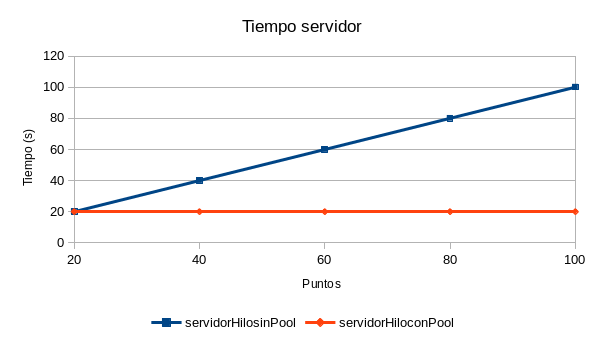
\includegraphics[scale=1]{TiempoServidor.png}
		\caption{Valores del tiempo del calculo de la integral de sen(x).}
		\label{fig:Valores del tiempo del calculo de la integral de sen(x)}
	\end{center}
\end{figure}
\noindent
En la tabla\footnote[1]{Para hacer la tabla de tiempos para el algoritmo \texttt{ServidorHiloconPool.java} hemos establecido un valor de TPool (tamaño del pool) de 20 elemntos.}, podemos ver que para el algoritmo \texttt{ServidorHilosinPool.java} el tiempo siempre va a ser el mismo debido a que las peticiones tardan un tiempo despreciable en comparación con el \texttt{sleep(1000)} que tiene en su código.\\

Sin embargo, para el algoritmo \texttt{ServidorHiloconPool.java} vemos que conforme vamos aumentando el número de peticiones, mayor va siendo el tiempo debido al tamaño del pool de threads y al número de peticiones. Por lo tanto, podemos obtener la siguiente fórmula que, para este caso, donde el tiempo que se tarda en procesar un hilo es prácticamente despreciable, nos dará el tiempo que tardará en procesarse los hilos que queramos en función del tamaño del pool:\\
\begin{center}
	$Tiempo = \lceil{\frac{NPeticiones\cdot 20}{TPool}}\rceil$
\end{center}
\newpage
Siendo:
\begin{itemize}
	\item \textbf{NPeticiones:} Es el número de peticiones que realiza el cliente. Queda establecido en el código de \texttt{ClienteMultiple.java}.
	\item \textbf{20:} Son los 20 segundos que tarda en procesarse una petición debido al \texttt{sleep(1000)} que tiene cada algoritmo en el \texttt{run} y que hace que en comparación con él, el tiempo que tarda en procesarse una iteración del hilo, sea, esta última, despreciable.
	\item \textbf{TPool:} Es el tamaño del pool de threads. Queda establecido en el código de \texttt{ServidorHiloconPool.java}.
\end{itemize}


\end{document}